\documentclass{article}

\usepackage[margin=1in]{geometry}
\usepackage{fancyhdr}
\usepackage{graphicx}
\usepackage{caption}
\usepackage{color}
\definecolor{bg}{rgb}{0.89, 0.95, 0.71} % background e3f3b4
\definecolor{ac}{rgb}{0.50, 0.18, 0.41} % accent c491b6
\definecolor{rc}{rgb}{0.77, 0.57, 0.71} % rule 7f2f69
\usepackage{url}
\usepackage[pdftex, 
            bookmarks, 
            colorlinks=true,
            linkcolor=black, 
            plainpages = false,
            pdfpagemode = UseNone,
            pdfstartview = FitH, 
            citecolor = ac, urlcolor = ac, filecolor = ac]{hyperref}
\usepackage[flushmargin]{footmisc}
\usepackage{enumerate}
\usepackage{listings}
\usepackage{subfigure}
\usepackage{tikz}

\usetikzlibrary{positioning, quotes, shapes}

\lstset{identifierstyle=\textbf,
        basicstyle=\ttfamily,
        aboveskip=\smallskipamount, belowskip=\medskipamount}
\lstloadlanguages{[ISO]C++}

\renewcommand{\footrulewidth}{0.4pt}% default is 0pt

% \newcounter{daggerfootnote}
% \newcommand*{\daggerfootnote}[1]{%
%     \setcounter{daggerfootnote}{\value{footnote}}%
%     \renewcommand*{\thefootnote}{\fnsymbol{footnote}}%
%     \footnote[2]{#1}%
%     \setcounter{footnote}{\value{daggerfootnote}}%
%     \renewcommand*{\thefootnote}{\arabic{footnote}}%
% }

\pagestyle{fancy}
\lhead{
\includegraphics[
            keepaspectratio=true,
            scale=0.022]{images/utm.png}}
\chead{\textit{Conferinţa Tehnico-Ştiinţifică a Studenţilor, Masteranzilor și Doctoranzilor,\\
Universitatea Tehnică a Moldovei}}
\rhead{\textbf{revized on \date{\today}}}
\lfoot{}
\cfoot{\textit{Chișinău, Republica Moldova, 27-29 martie 2024, Vol. II}\\ \thepage}
\rfoot{\LaTeX}

\title{FORMALIZATION OF DISTRIBUTED SYSTEMS WITH SEMANTIC
INTEROPERABILITY}
\author{Leon BRÂNZAN\thanks{Departamentul Informatică și Ingineria Sistemelor, Facultatea Calculatoare, Informatică și Microelectronică, Universitatea Tehnică a Moldovei, Chișinău, Republica Moldova} \\ \href{mailto:leon.branzan@doctorat.utm.md}{\texttt{leon.branzan@doctorat.utm.md}}}
\date{March, 29th, 2024}


\begin{document}
\maketitle

\begin{abstract}
    Distributed software systems have been designed, studied, and implemented for decades, yet problems with their development, deployment, and maintenance persist even today. Attempts
    at formalizing the crucial concepts of distributed systems often lead nowhere or fail outright, as is
    demonstrated in this article.

    A hypothesis is then proposed: using mathematical models dealing with semantics of interoperability
    of systems it is possible to develop a better understanding of distributed computing using not the objects
    within the system, but the relations between these objects. The article describes a use case for applying
    semantic analysis to solve persisting problems with industrial systems.

    Viable solutions to these problems are then suggested, borrowed from well-formalized
    mathematical theories, such as domain theory and category theory. The article attempts to
    partially answer the questions it poses using “semantic interoperability”---the property of a
    notation to have different formal definitions of the same concept be fully interchangeable in the
    context of a unifying formal description. 
    \end{abstract}
    \textit{\textbf{Keywords}: denotational semantics; category theory; distributed systems; network architecture.}

\tableofcontents

\newpage

\section*{Introduction}
\addcontentsline{toc}{section}{\protect\numberline{}Introduction}

On March 5th, 2024, Facebook, Instagram, Threads, and several other communication
services developed by Meta suffered a global outage, resulting in millions of people losing access
to their accounts for the duration of the outage \cite{Rita}. It is speculated that the core issue lied with the
company’s internal network infrastructure. This was not the first time such an event took place.
On October 4th, 2021, a massive outage disrupted Meta’s services globally. In a post-mortem \cite{Janardhan}
Meta’s engineers narrowed down the issues to an error with DNS configuration. Such episodes are
not specific to Meta, nor are they rare. Distributed systems “are hard” \cite{Kingsbury}.

The problem here is not with the systems themselves. Engineers dedicate a lot of man-hours making sure such systems stay available and reliable. Rather, the problem is the over-reliance on private systems for global communication, oftentimes in critical moments \cite{Davies}. The
Internet was initially developed as an open network, and communication was and still is its primary
function. Communication channels should not be gated by private entities. Specifically,
international communication should be subject to international law. It is difficult to police private
companies outside of one’s authority in cases when said companies fail to comply with local laws,
especially since it is much easier for private entities to deny their services rather than litigate.
Global communication relies almost entirely on independent entities, critical infrastructure that
millions depend on is out of most people’s reach.

When large companies like Amazon, Meta etc. cannot fix the issues with stability of their
systems, it is a good indicator that these problems cannot be fixed just with money. Networks
created on top of the Internet must be aware of the underlying infrastructure and replicate its most
important properties.

\section*{Centralized networks in a decentralized architecture}
\addcontentsline{toc}{section}{\protect\numberline{}Centralized networks in a decentralized architecture}

The World Wide Web was initially devised as a network for exchanging texts between
scientific institutions \cite{Lee1}. But even then, its designer Tim Berners-Lee considered it just an initial
step, and the future of the network to be in machines communicating with other machines \cite{Lee2}.
XML was one of the formats intended to bridge that gap. But instead, social networks took over
and are still omnipresent. Even though the phenomenon, which is today known under the name
“Web 2.0”, came about as the result of multiple efforts to democratize the process of publishing
content on web sites \cite{Sykora}, its arguably biggest impact lies in concentrating most human
communication within several private centralized networks; the other important aspect of this
process is the noticeable effect that mainstream advertising practices have on the nature of content
published on the biggest social networks \cite{Walter}.

As illustrated in “The Semantic Web” \cite{Lee1}, the future of the World Wide Web looked
different to its creators and early adopters. That future was based on evolving the way various
entities within the Web exchanged information (a good example of that view is Szabo’s seminal
work on secure information exchange on public networks \cite{Szabo}), closer in its architecture to a huge
peer-to-peer network. Today, most of the Web’s communication is orchestrated by huge
centralized systems. All the while peer-to-peer networks are reserved for hobbyists; federated
communication networks outside email are considered niche.

One would expect a significant shift in this paradigm with the advent of the Internet of
Things. This model seems to mimic the kind of architecture described in “The Semantic Web.” It
is often just a replication of already existing architectures (most of which originate in social
networks; for example, Software-as-a-Service monetization schemes being prevalent in IoT
solutions, with companies denying services at their convenience \cite{Acoba,Gitlin,Hamzelou}). On the surface, IoT
should be an integral part of the Internet, seemingly inseparable. If Internet service is available,
the device should be fully functional. Currently, when the company ceases to service or update
their product, it becomes unusable.

There are attempts at changing the status quo. Several protocols and implementations have
been proposed in the last 5--10 years, with their adoption lagging behind. ActivityPub is one such
example \cite{Lemmer}, its mission being rebuilding the Web as a decentralized system, as it was imagined
before “everything got locked down into a handful of walled gardens”. Notable implementations
are Mastodon and Blue Sky. Another example, which aims to “radically change the way Web
applications work today, resulting in true data ownership as well as improved privacy”, is Solid---a project headed by Berners-Lee himself \cite{Mansour}.

An alternative approach to solving this problem would be to change the underlying
software in a way that would compel users to change their behavior. This can be traced in how
such changes in behavior were happening before: a new way to interact with the system would be
identified, adopted by a small group of people, gain critical mass and then explode in popularity\footnote{This process is sometimes referred to as “Crossing the Chasm”, a phrase coined by G. A. Moore.}.
Web 2.0 is a good illustration of this process. from an engineering perspective developing a new
system for enacting a similar shift would be an insurmountable task even for a group of developers,
let alone one person. A different strategy needs to be adopted. Instead of creating an unproven
system and then expecting it to eventually do what it was designed to do, another approach would
be to first prove that such a system is:
\begin{enumerate}[a.]
\item viable;
\item capable of changes expected of it;
\item will work according to its specification.
\end{enumerate}
A rigorous proof would require a precise formal description (existing or new). Considering
the nature of distributed systems, describing a proof concerning relations between objects in such
a system would require either developing a new general formal language or finding a way of
unifying existing formalisms (syntactic models) for describing distributed systems (e. g. Erlang’s “Actor” model \cite{Hewitt}). One possible approach could be based on generalizing different models using
a more abstract notion of relations between objects.

\section*{Computation and storage}
\addcontentsline{toc}{section}{\protect\numberline{}Computation and storage}

Distributed systems research revolves around computation and storage. A lot of mainstream
research is focused on large text processing, consensus protocols, data replication, and performance\footnote{This assumption is based on MIT’s 2023 curriculum for the “Distributed Systems” course, which is
available at \href{https://pdos.csail.mit.edu/6.824/schedule.html}{pdos.csail.mit.edu}.}.
In the curriculum the gap between early research papers and modern research topics is noticeably
large (this could be attributed, at least in part, to COVID-19). Still, a lot of effort has been spent over
the decades to formalize certain aspects of distributed systems, sometimes with unexpected results.

One rather contentious topic in distributed systems design is the CAP\footnote{CAP is an acronym that stands for “\textbf{c}onsistency, \textbf{a}vailability, \textbf{p}artitions”.} theorem \cite{Gilbert}. The
original conjecture \cite{Brewer} states, in plain terms, that it is possible to “have at most two of these
properties for any shared-data system:
\begin{enumerate}[-]
    \item consistency;
    \item availability;
    \item tolerance to network partitions.”
\end{enumerate}
The theorem garnered a lot of exposure and critique \cite{Kleppmann1,Tornow}. Famously, Kleppmann once
noted that, “the CAP theorem is too simplistic and too widely misunderstood to be of much use
for characterizing systems. Therefore I ask that we retire all references to the CAP theorem, stop
talking about the CAP theorem, and put the poor thing to rest” \cite{Kleppmann2}. Invariant Confluence \cite{Bailis} is
proposed by many as a viable alternative.

Both approaches formalize data consistency when synchronized over a network. The other
important topic is network consensus. Two major results in this domain are Paxos \cite{Lamport} and
Viewstamped Replication \cite{Oki}. While the former is more widely known, there are well-documented
attempts at making it “more approachable” for developers, garnering the algorithm a reputation of
being difficult to implement. The more recent Raft algorithm implements Viewstamped Replication
with several new features \cite{Ongaro} and should be considered over older consensus algorithms.

The research discussed above shows that distributed systems formalization is an important
topic, and that there are many problems in distributed systems design, that are still unsolved. One
of the preliminary conclusions of this paper is the assumptions that the Internet’s properties and
processes need to be formalized to make their replication and adoption in higher-level architectures
more widespread and systematic. The focus, then, is on how distributed systems orchestrate
communication between its actors, depending on the architecture (decentralized, federated, peer-to-peer, or hybrid). The intuition is: to see how that could work it would be beneficial to look at
distributed systems from “a bird’s eye view”---one level of abstraction higher.

\section*{Semantic interoperability}
\addcontentsline{toc}{section}{\protect\numberline{}Semantic interoperability}

The “semantics” of a system is its behavior. From a broad point of view, semantics and
realization are aspects of the same situation: semantics is the problem of system analysis; while
realization is the problem of system synthesis \cite{Goguen1}. In general, semantics are separated into three
major classes:
\begin{enumerate}
    \item \textbf{Operational}. Meanings for program phrases defined in terms of the steps of
    computation they can take during program execution.
    \item \textbf{Axiomatic}. Meanings for program phrases defined indirectly via the axioms and rules
    of some logic of program properties.
    \item \textbf{Denotational}. Concerned with giving mathematical models of programming
    languages. Meanings for program phrases defined abstractly as elements of some
    suitable mathematical structure.
\end{enumerate}
When attempting to look at concrete things closely, having a formal way of abstracting all
the details would help immensely. Researchers often turn to formalization while looking for viable
solutions to concrete problems. When formalizing distributed informational systems one important
property that needs to be preserved is semantic interoperability---“what is sent is what is
understood” (for the purposes of this text semantic interoperability is defined as in \cite{Miscena}).

Consider the issues that could arise from fragmenting distributed networks along the
connections inside them. Such division will inevitably make a network heterogeneous, which
immediately leads to several problems that need to be addressed \cite{Mello}: data incompatibility, the
need for APIs at each point of connection, new metadata schemas etc.

One concrete example would be the Internet of Things. While each device can be connected
to the internet and have a well-defined human-machine interface, things can quickly break down
when attempting to make two devices communicate with each other (see “smart objects” \cite{Novo} for
one proposed solution).

Another example is programming language interoperability. Languages have the extra
burden of syntactic interoperability and semantic interoperability. Existing solutions often revolve
around creating a language extension or a language framework to overcome this issue. Other
solutions attempt to formalize the higher-level concepts of a language (see “linear language
interoperability” \cite{Scherer} for one proposed solution).

One example of an interoperable formal description of a property of a distributed system
is MixT \cite{Milano}---a C++-derived transaction language for concurrent computations, that enables its
type system (and the compiler by extension) to catch incorrect formalisms. It is partially based on
the concept of full abstraction borrowed from denotational semantics.

Listing \ref{mixtc} represents a language embedding designed to solve issues with concurrent mutation---the iterator in the fragment on the left can be invalidated by one thread while another is accessing its value. To combat this, a “transaction block” is introduced with the \lstinline{mixt_method} declaration. Such blocks are context-aware, which allows them to safely merge concurrent operations, ensuring
causal consistency.
    
\noindent\begin{minipage}[h]{.35\textwidth}
    \begin{lstlisting}[basicstyle=\footnotesize,
            stringstyle=\ttfamily,
            language={[ISO]C++}, frame=single,
            abovecaptionskip=\smallskipamount,
            title=(a) Unsafe C++ code, label=mixtl]
var iterator = users, 
while (iterator.isValid()) {
    log.append(iterator->v
    .inbox.insert(post)),
    iterator = iterator->next
}
    \end{lstlisting}
\end{minipage}\hfill
\begin{minipage}[h]{.63\textwidth}
    \begin{lstlisting}[basicstyle=\footnotesize,
                stringstyle=\ttfamily,
                language={[ISO]C++}, frame=single,
                abovecaptionskip=\smallskipamount,
                title=(b) Code embedded within a MixT structure, label=mixtr]
class User {
    Handle<set<string>>, causal, supports<insert>> inbox;
    };
    
class group {
    RemoteList<Handle<user, causal>, linearizable> users;
    Handle<Log, eventual, supports<append>> log;
    mixt_method(add_post) (post) mixt_captures(users, log) 
    (...)
};
    \end{lstlisting}
\end{minipage}
\captionof{lstlisting}{\label{mixtc}MixT language embedding\cite{Milano}\\}

To summarize, denotational semantics serve “to specify programming language constructs
in as abstract and implementation-independent way as possible: in this way one may gain insight
into the fundamental concepts underlying programming languages, their inter-relationships, and
(sometimes) new ways of realising those concepts in language designs \cite{Scott}.”

\section*{Categories}
\addcontentsline{toc}{section}{\protect\numberline{}Categories}

Another mathematical theory that deals in abstractions and uses mathematical concepts to
describe all sorts of entities is category theory. It is being widely used in modern research to
explain different phenomena that were hard or impossible to describe using other methods.

It is outside of the scope of this paper to include a section on the basics of category theory,
for a detailed illustrated introduction refer to \cite{Tsuchiya}. Below is a diagram describing three main
mathematical properties of an object that qualify it as a category (see fig. \ref{catprop}).

\begin{figure}[h]
    \begin{center}
        \subfigure[Composition]{
            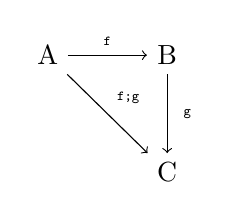
\begin{tikzpicture}[
                    every node/.style = {text=black, minimum width = 0.5cm},
                    every edge/.style = {draw,->},
                    every edge quotes/.style = {auto, font=\tiny\ttfamily, text=black}]
                \node (o) [text=white, fill=white] {O};
                \node (c) [fill=white,right = of o] {C};
                \node (a) [fill=white, above = of o] {A};
                \node (b) [fill=white, above = of c] {B};
                \draw (a) edge["f"]    (b);
                \draw (a) edge["f;g"] (c);
                \draw (b) edge["g"]   (c);
            \end{tikzpicture}
        }
        \subfigure[Associativity]{
            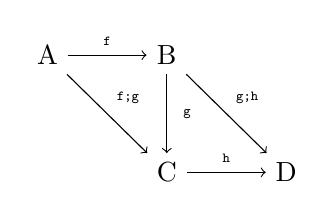
\begin{tikzpicture}[
                    every node/.style = {text=black, minimum width = 0.5cm},
                    every edge/.style = {draw,->},
                    every edge quotes/.style = {auto, font=\tiny\ttfamily, text=black}]
                \node (d) [text=white, fill=white]   {D};
                \node (c) [fill=white,right = of d]  {C};
                \node (a) [fill=white, above = of d] {A};
                \node (b) [fill=white, above = of c] {B};
                \node (d) [fill=white, right = of c] {D};
                \draw (a) edge["f"]   (b);
                \draw (a) edge["f;g"] (c);
                \draw (b) edge["g"]   (c);
                \draw (c) edge["h"]   (d);
                \draw (b) edge["g;h"] (d);
            \end{tikzpicture}
        }
        \subfigure[Identity (unit)]{
            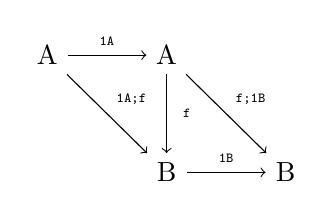
\begin{tikzpicture}[
                    every node/.style = {text=black, minimum width = 0.5cm},
                    every edge/.style = {draw,->},
                    every edge quotes/.style = {auto, font=\tiny\ttfamily, text=black}]
                \node (d) [text=white, fill=white]   {B};
                \node (c) [fill=white,right = of d]  {B};
                \node (a) [fill=white, above = of d] {A};
                \node (b) [fill=white, above = of c] {A};
                \node (d) [fill=white, right = of c] {B};
                \draw (a) edge["1A"]   (b);
                \draw (a) edge["1A;f"] (c);
                \draw (b) edge["f"]    (c);
                \draw (c) edge["1B"]   (d);
                \draw (b) edge["f;1B"] (d);
            \end{tikzpicture}
        }
    \end{center}
    \caption{Illustration of three basic properties of a category \cite{Tsuchiya}.}
    \label{catprop}
\end{figure}

Even though category theory is often called “abstract nonsense,” it has real application in many
domains. One example is using the Yoneda lemma---one of the foundational theorems of category
theory. To understand the core of the Yoneda lemma: in simple terms, imagine a deck of playing cards.
If one person picks a random card and asks another person to guess it by asking questions about it, it
would be possible to pin down the card in a finite number of questions (for example, questions like “is
it a spade?”, “is it higher than a 10?” etc. will eventually lead to the correct card by elimination). In
even plainer terms, it is possible to define an object by its relation to other objects definitively. Figure \ref{qual} presents a visual reference for the “Inverted spectrum” problem \cite{Byrne}.

% qualia.gif
\begin{figure}[h]
    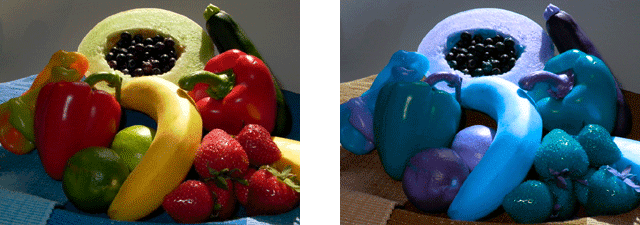
\includegraphics[
        scale=0.5,
        width=\linewidth]{images/qualia.png}
    \caption{Illustration of the "inverted spectrum" problem \cite{Byrne}.}
    \label{qual}
\end{figure}

If two people look at the same set of objects and are asked to name the objects’ colors, both
will name the same colors, even when one of the persons has color vision deficiency. That person
will have grown up with knowing a certain color as “red,” even though it would not necessarily
qualify as “red” on the color spectrum. The Yoneda lemma gives a solution to this. Figure \ref{spectr} shows
the illustrated solution to the “Inverted spectrum” problem.

\begin{figure}[h!]
    \begin{center}
        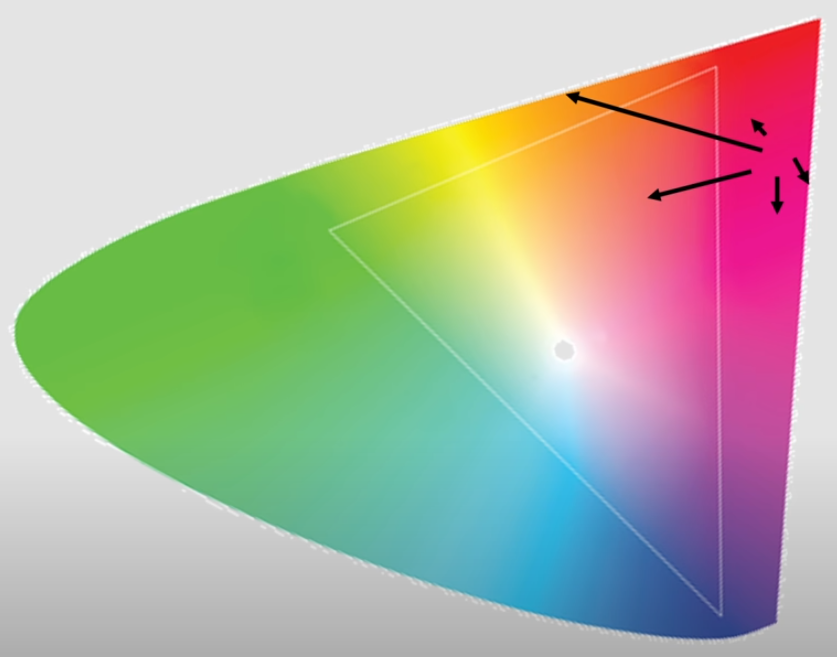
\includegraphics[
        % scale=0.5,
        width=0.5\linewidth,
        keepaspectratio=true]{images/spectrum.png}
    \end{center}
    \caption{Human color perception as a distorted space \cite{Maier}.}
    \label{spectr}
\end{figure}

By transforming the color spectrum into a distorted space, the problem can be reframed as
a mathematical problem. Any point of that space can be determined in terms of its relations with
all other points of the space. Any point considered being in the red spectrum will have only one
way of defining it in terms of all other points. Thus, any person not seeing it in the red part of the
spectrum can be identified.

\section*{Conclusions}
\addcontentsline{toc}{section}{\protect\numberline{}Conclusions}

Another important concept of category theory is that of a functor. Without going into too
much detail, a functor represents transformations between categories in the same way that
functions are transformations between objects within a category (in this case---a set). Functors
have one important property that is pertinent to this paper’s subject. Applying a functor to a
composition of two transformations is equivalent to applying a functor to each transformation
separately and then composing the results \cite{Ahrens}. This is illustrated as a diagram below (see fig. \ref{funct}).

% functor diagram
\begin{figure}[h]
    \begin{center}
        \subfigure{
            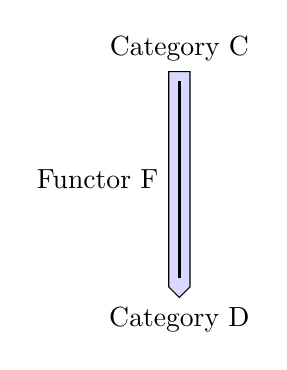
\begin{tikzpicture}
                \node [ signal,
                        label=left:Functor F,
                        label=above:Category C,
                        label=below:Category D,
                        draw, 
                        fill=blue!15, signal to=south, anchor=west] {
                    \vrule width 1pt height 2.5cm};
            \end{tikzpicture}
        }
        \subfigure{
            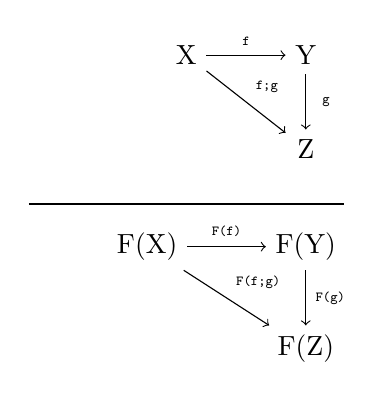
\begin{tikzpicture}[
                    every node/.style = {text=black, minimum width = 0.5cm},
                    every edge/.style = {draw,->},
                    every edge quotes/.style = {auto, font=\tiny\ttfamily, text=black}]
            \begin{scope}[node distance=0.7cm and 1cm]
                \node (o) [text=white, fill=white] {O};
                \node (c) [fill=white, right = of o] {Z};
                \node (a) [fill=white, above = of o] {X};
                \node (b) [fill=white, above = of c] {Y};

                \draw (a) edge["f"]   (b);
                \draw (a) edge["f;g"] (c);
                \draw (b) edge["g"]   (c);

                \draw [thick] (-2,-0.7) -- (2,-0.7);

                \node (g) [fill=white, below = of c] {F(Y)};
                \node (e) [fill=white, below = of g] {F(Z)};
                \node (f) [fill=white, left = of g] {F(X)};

                \draw (f) edge["F(f)"]   (g);
                \draw (f) edge["F(f;g)"] (e);
                \draw (g) edge["F(g)"]   (e);
            \end{scope}
            \end{tikzpicture}
        }
    \end{center}
    \caption{Functor preserving commuting and composition \cite{Ahrens}.}
    \label{funct}
\end{figure}

This can be applied to describing how two heterogeneous systems interface with each other.
If there are two systems that are connected to each other somehow, having some operations
available in one system, it should give the same result in both cases:
\begin{enumerate}[*]
    \item Operations are combined (read, performed one immediately after another “piping” the
    intermediate result between them), and then the end result is transported to the other
    system.
    \item Operations themselves are transported into the other system and combined there.
\end{enumerate}
Meaning, that if both systems formally guarantee that the operations and objects possess
certain properties, functors have the explanatory power to guarantee consistency of data between
heterogeneous systems.

This is just one example of how category theory could be leveraged for designing and
describing complex interconnected systems. In that the author of this paper agrees with Joseph
Goguen, “computing science is very fragmented, with many different sub-disciplines having many
different schools within them. Hence, we badly need the kind of conceptual unification that
category theory can provide \cite{Goguen2}”.

Of course, the path to unification need not lie in category theory necessarily. But it would be
a good first step, because concepts developed using category theory are easily generalized and can
rely on many mathematical proofs to ensure that what they describe they do with enough precision.
To quote Scott and Strachey again, “there are many different languages adequate for conveying the
same concepts (e.g., binary, octal, or decimal numerals). Even in the same language many different
expressions can denote the same concepts (e.g., $2+2$, $4$, $1+1+1+1$, etc.). The problem of explaining
these equivalences of expressions (whether the same or different languages) is one of the tasks of
semantics and is much too important to be left to syntax alone. Besides, the mathematical concepts
are required for the proof that the various equivalences have been correctly described \cite{Scott}.”




\begin{thebibliography}{99}
    \bibitem{Rita}
    A. Rita, “Facebook Service Outage Postmortem,” Medium. Accessed: Apr. 10, 2024. [Online]. Available: \href{https://medium.com/@egwuaturita95/facebook-service-outage-
    postmortem-479cd1a3a6f8}{medium.com}.

    \bibitem{Janardhan}
    S. Janardhan, “More details about the October 4 outage,” Engineering at Meta. Accessed:
    Apr. 10, 2024. [Online]. Available: \href{https://engineering.fb.com/2021/10/05/networking-
    traffic/outage-details/}{engineering.fb.com}.

    \bibitem{Kingsbury}
    K. Kingsbury, “The network is reliable,” Aphyr. Accessed: Apr. 10, 2024. [Online]. Available: \href{https://aphyr.com/posts/288-the-network-is-reliable}{aphyr.com}.

    \bibitem{Davies}
    D. Davies, “Social media’s role in Jan. 6 was left out of the final report,” NPR. Accessed: Apr. 10, 2024. [Online]. Available: \href{https://www.npr.org/2023/01/26/1151360750/social-medias-role-in-jan-6-was-left-out-of-the-final-report}{npr.org}.

    \bibitem{Lee1}
    T. Berners-Lee, “Information Management: A Proposal,” CERN, TBL-900620, May 1990.

    \bibitem{Lee2}
    T. Berners-Lee, J. Hendler, and O. Lassila, “The Semantic Web: A New Form of Web Content that is Meaningful to Computers will Unleash a Revolution of New Possibilities,” in Linking the World’s Information, 1st ed., O. Seneviratne and J. Hendler, Eds., New York, NY, USA: ACM, 2001, pp. 91–103. doi: 10.1145/3591366.3591376.

    \bibitem{Sykora}
    M. Sykora, “Web 1.0 to Web 2.0: an observational study and empirical evidence for the historical r(evolution) of the social web,” IJWET, vol. 12, no. 1, p. 70, 2017, doi: 10.1504/IJWET.2017.084024.

    \bibitem{Walter}
    Y. Walter, “Artificial influencers and the dead internet theory,” AI \& Soc, Feb. 2024, doi: 10.1007/s00146-023-01857-0.

    \bibitem{Szabo}
    N. Szabo, “Formalizing and Securing Relationships on Public Networks,” First Monday, vol. 2, no. 9, Sep. 1997, [Online]. Available: \href{https://firstmonday.org/ojs/index.php/fm/article/view/548/469}{firstmonday.org}.
    
    \bibitem{Acoba}
    P. Acoba, “Tesla allegedly remotely unlocks Model 3 owner’s car, uses smart summon to help repo agent,” Tire Meets Road. Accessed: Apr. 10, 2024. [Online]. Available: \href{https://tiremeetsroad.com/2021/03/18/tesla-allegedly-remotely-unlocks-model-3-owners-
    car-uses-smart-summon-to-help-repo-agent/}{tiremeetsroad.com}.

    \bibitem{Gitlin}
    J. M. Gitlin, “John Deere relents, says farmers can fix their own tractors after all,” Ars Technica. Accessed: Apr. 10, 2024. [Online]. Available: \href{https://arstechnica.com/tech-
    policy/2023/01/john-deere-relents-says-farmers-can-fix-their-own-tractors-after-all/}{arstechnica.com}.

    \bibitem{Hamzelou}
    J. Hamzelou, “A brain implant changed her life. Then it was removed against her will,” MIT Technology Review. Accessed: Apr. 10, 2024. [Online]. Available: \href{https://www.technologyreview.com/2023/05/25/1073634/brain-implant-removed-against-
her-will/}{technologyreview.com}.

    \bibitem{Lemmer}
    C. Lemmer-Webber, J. Tallon, E. Shepherd, A. Guy, and E. Prodromou, “ActivityPub,”
W3C, Recommendation REC-activitypub-20180123, Jan. 2018. Accessed: Apr. 10, 2024.
[Online]. Available: \href{https://www.w3.org/TR/activitypub/}{w3.org}.

    \bibitem{Mansour}
    E. Mansour et al., “A Demonstration of the Solid Platform for Social Web Applications,” in Proceedings of the 25th International Conference Companion on World Wide Web---WWW ’16 Companion, Montreal, Quebec, Canada: ACM Press, 2016, pp. 223–226. doi: 10.1145/2872518.2890529.

    \bibitem{Hewitt}
    C. Hewitt, “Actor Model of Computation.” arXiv, Nov. 07, 2010. doi: \href{https://doi.org/10.48550/arXiv.1008.1459}{10.48550/arXiv.1008.1459}.

    \bibitem{Gilbert}
    S. Gilbert and N. Lynch, “Brewer’s Conjecture and the Feasibility of Consistent, Available, Partition-Tolerant Web Services,” SIGACT News, vol. 33, no. 2, pp. 51–59, Jun. 2002, doi: 10.1145/564585.564601.

    \bibitem{Brewer}
    E. A. Brewer, “Towards robust distributed systems (abstract),” in Proceedings of the nineteenth annual ACM symposium on Principles of distributed computing, in PODC ’00. Portland Oregon USA: ACM, Jul. 2000, p. 7. doi: 10.1145/343477.343502.

    \bibitem{Kleppmann1}
    M. Kleppmann, “A Critique of the CAP Theorem.” arXiv, Sep. 18, 2015. Accessed: Mar. 09, 2024. [Online]. Available: \href{http://arxiv.org/abs/1509.05393}{arxiv.org/abs/1509.05393}.

    \bibitem{Tornow}
    D. Tornow, “The CAP Theorem. The Bad, the Bad, \& the Ugly,” DTornow. Accessed: Apr. 04, 2024. [Online]. Available: \href{https://blog.dtornow.com/the-cap-theorem.-the-bad-
    the-bad-the-ugly/}{blog.dtornow.com}.

    \bibitem{Kleppmann2}
    M. Kleppmann, “Please stop calling databases CP or AP,” Martin Kleppmann. Accessed: Apr. 10, 2024. [Online]. Available: \href{https://martin.kleppmann.com/2015/05/11/please-stop-calling-databases-cp-or-ap.html}{martin.kleppmann.com}.

    \bibitem{Bailis}
    P. Bailis, A. Fekete, M. J. Franklin, A. Ghodsi, J. M. Hellerstein, and I. Stoica, “Coordination avoidance in database systems,” Proc. VLDB Endow., vol. 8, no. 3, pp. 185–196, Nov. 2014, doi: 10.14778/2735508.2735509.

    \bibitem{Lamport}
    L. Lamport, “The Part-Time Parliament,” ACM Transactions on Computer Systems, vol. 16, no. 2, pp. 133–169, May 1998, doi: 10.1145/279227.279229.

    \bibitem{Oki}
    B. Oki and B. Liskov, “Viewstamped Replication: A New Primary Copy Method to Support Highly-Available Distributed Systems,” in Proceedings of the Seventh Annual ACM Symposium on Principles of Distributed Computing, in PODC ’88. Toronto, Ontario, Canada: Association for Computing Machinery, 1988, pp. 8–17. doi: 10.1145/62546.62549.

    \bibitem{Ongaro}
    D. Ongaro and J. Ousterhout, “In Search of an Understandable Consensus Algorithm,” in 2014 USENIX Annual Technical Conference, Stanford University: USENIX Association, Jun. 2014, pp. 305-319. Accessed: Apr. 10, 2024. [Online]. Available: \href{https://www.usenix.org/conference/atc14/technical-sessions/presentation/ongaro}{usenix.org}.

    \bibitem{Goguen1}
    J. A. Goguen, “Semantics of Computation,” Computer Science \& Engineering. Accessed: Apr. 10, 2024. [Online]. Available: \href{https://cseweb.ucsd.edu/~goguen/projs/sem.html}{cseweb.ucsd.edu}.

    \bibitem{Miscena}
    E. Miscena and C. de Guerdavid, Eds., “European Interoperability Framework:
    Implementation Strategy.” National Interoperability Framework Observatory, Mar. 23,
    2017. Accessed: Apr. 10, 2024. [Online]. Available: \href{https://joinup.ec.europa.eu/collection/nifo-national-interoperability-framework-
    observatory/glossary/term/semantic-interoperability}{joinup.ec.europa.eu}.

    \bibitem{Mello}
    B. H. De Mello et al., “Semantic interoperability in health records standards: a systematic literature review,” Health Technol., vol. 12, no. 2, pp. 255–272, Mar. 2022, doi: 10.1007/s12553-022-00639-w.

    \bibitem{Novo}
    O. Novo and M. D. Francesco, “Semantic Interoperability in the IoT: Extending the Web
    of Things Architecture,” ACM Trans. Internet Things, vol. 1, no. 1, pp. 1–25, Feb. 2020,
    doi: 10.1145/3375838.

    \bibitem{Scherer}
    G. Scherer, M. New, N. Rioux, and A. Ahmed, “FabULous Interoperability for ML and a
    Linear Language.” arXiv, Apr. 12, 2018. Accessed: Feb. 29, 2024. [Online]. Available: \href{http://arxiv.org/abs/1707.04984}{arxiv.org/abs/1707.04984}.

    \bibitem{Milano}
    M. Milano and A. C. Myers, “MixT: a language for mixing consistency in geodistributed
    transactions,” in Proceedings of the 39th ACM SIGPLAN Conference on Programming
    Language Design and Implementation, Philadelphia PA USA: ACM Press, Jun. 2018, pp.
    226–241. doi: 10.1145/3192366.3192375.

    \bibitem{Scott}
    D. Scott and C. Strachey, “Toward a Mathematical Semantics for Computer Languages,”
    Oxford University, Oxford University Computer Laboratory Programming Research
    Group, Monograph PRG-6, Oct. 1971. [Online]. Available: \href{https://www.cs.ox.ac.uk/publications/publication3723-abstract.html}{cs.ox.ac.uk}.

    \bibitem{Tsuchiya}
    N. Tsuchiya and H. Saigo, “A relational approach to consciousness: categories of level
    and contents of consciousness,” Neuroscience of Consciousness, vol. 2021, no. 2, Aug.
    2021, doi: 10.1093/nc/niab034.

    \bibitem{Byrne}
    A. Byrne, “Inverted Qualia,” Stanford Encyclopedia of Philosophy. Accessed: Apr. 10,
    2024. [Online]. Available: \href{https://plato.stanford.edu/entries/qualia-inverted/}{plato.stanford.edu}.

    \bibitem{Maier}
    A. Maier, “Category Theory for Neuroscience (pure math to combat scientific
    stagnation)”. Accessed: Apr. 10, 2024. [Presentation]. Available: \href{https://www.youtube.com/watch?v=4GJ4UQZvCNM}{youtube.com}.

    \bibitem{Ahrens}
    B. Ahrens, C. Kapulkin, and M. Shulman, “Univalent categories and the Rezk
    completion,” Math. Struct. Comp. Sci., vol. 25, no. 5, pp. 1010–1039, Jun. 2015, doi:
    10.1017/S0960129514000486.

    \bibitem{Goguen2}
    J. A. Goguen, “A categorical manifesto,” Math. Struct. Comp. Sci., vol. 1, no. 1, pp. 49–
    67, Mar. 1991, doi: 10.1017/S0960129500000050.

\end{thebibliography}



\end{document}
